\newpage
\mysection{Array Based Binary Tree}\label{abbst}\hypertarget{abbst}{}

When storing values in an array as if it were a \gls{bintree}, you use the current location: \textbf{i} and multiply it by 2 for the location of the left child, or multiply by 2 and add 1 for the location of the right child. For this reason, we ignore the $0^{th}$ location in the array, since zero multiplied by anything is ... well ... zero. \\

The table below shows us the calculations for \textit{Left Child}, \textit{Right Child}, and \textit{Parent} in the left column. The right column gives a visual example in which we can see that index \textbf{7} would have \textbf{3} as its parent ($i/2$ or $7/3$) and the left and right children of index \textbf{5} are \textbf{10} and \textbf{11} respectively ($2*5$ and $2*5+1$).

\mysubsubsection{Formulas}

\begin{center}
\begin{tabular}{|M{0.30\textwidth}|M{0.60\textwidth}|}
\hline
\textbf{Formulas} & \textbf{Visualization}\\
\hline
\begin{itemize}
\tightlist
\item Left Child \hspace{4.5mm}= $2 * i$
\item Right Child  \hspace{2mm}= $2 * i + 1$
\item Parent \hspace{1cm}= $i / 2$
\end{itemize}&
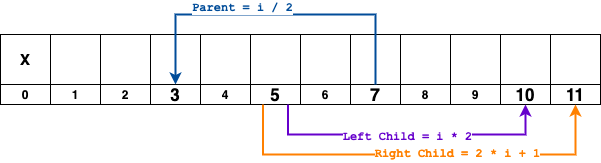
\includegraphics[scale=.4]{images/binary_tree_array_traversing.png} \\
\hline
\end{tabular}
\end{center}

\mysubsubsection{Example}
Below is an example inserting the values 13, 7 , 3, 17, 5, 11, 23 into an array based tree, along with it's binary tree equivalent. 

\begin{center}
\begin{tabular}{|M{0.10\textwidth}|M{0.50\textwidth} M{0.35\textwidth}|}
\hline
\textbf{Event} & \textbf{Array Based Tree} & \textbf{Binary Tree}\\
\hline
Insert 13 & 
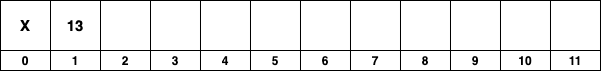
\includegraphics[scale=.4]{images/binary_tree_array_01.png} & 
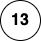
\includegraphics[scale=.4]{images/binary_tree_example_01.png}\\
& \footnotesize{The root of the tree is empty. So location \textbf{1} gets the value.} &   \\
\hline
\end{tabular}
\end{center}
\begin{center}
\begin{tabular}{|M{0.10\textwidth}|M{0.50\textwidth} M{0.35\textwidth}|}
\hline
Insert 7 &
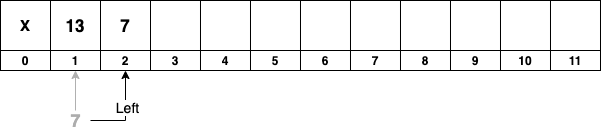
\includegraphics[scale=.4]{images/binary_tree_array_02.png} & 
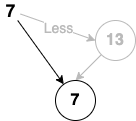
\includegraphics[scale=.4]{images/binary_tree_example_02.png}\\
& \footnotesize{7 is less than 13, go left. Its empty, store it there.} &   \\
\hline
\end{tabular}
\end{center}
\begin{center}
\begin{tabular}{|M{0.10\textwidth}|M{0.50\textwidth} M{0.35\textwidth}|}
\hline
Insert 17 &
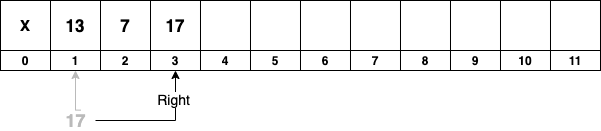
\includegraphics[scale=.4]{images/binary_tree_array_03a.png} & 
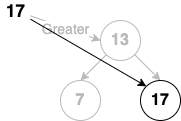
\includegraphics[scale=.4]{images/binary_tree_example_03.png}\\
& \footnotesize{17 is greater than 13, go right. Its empty, store it there.} &   \\
\hline
\end{tabular}
\end{center}
\begin{center}
\begin{tabular}{|M{0.10\textwidth}|M{0.50\textwidth} M{0.35\textwidth}|}
\hline
Insert 3 &
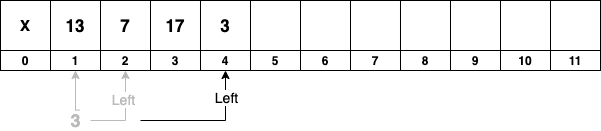
\includegraphics[scale=.4]{images/binary_tree_array_04a.png} & 
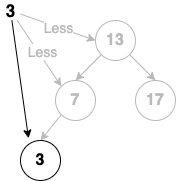
\includegraphics[scale=.4]{images/binary_tree_example_04.png}\\
& \footnotesize{3 is less than 13, go left. 3 is less than 7, go left. Its empty, store it there.} &   \\
\hline
\end{tabular}
\end{center}
\begin{center}
\begin{tabular}{|M{0.10\textwidth}|M{0.50\textwidth} M{0.35\textwidth}|}
\hline
Insert 5 &
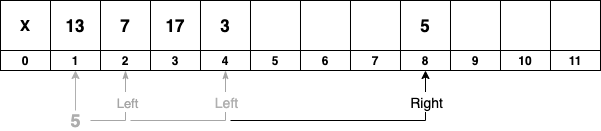
\includegraphics[scale=.4]{images/binary_tree_array_05.png} & 
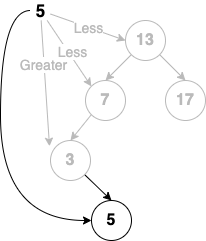
\includegraphics[scale=.4]{images/binary_tree_example_05.png}\\
& \footnotesize{5 is less than 13, go left. 5 is less than 7, go left. 5 is greater than 3, go right. Its empty, store it there.} &   \\
\hline
\end{tabular}
\end{center}
\begin{center}
\begin{tabular}{|M{0.10\textwidth}|M{0.50\textwidth} M{0.35\textwidth}|}
\hline
Insert 11 &
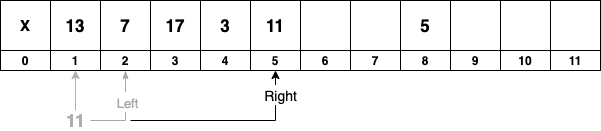
\includegraphics[scale=.4]{images/binary_tree_array_06.png} & 
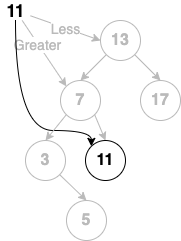
\includegraphics[scale=.4]{images/binary_tree_example_06.png}\\
& \footnotesize{11 is less than 13, go left. 11 is greater than 7, go right. Its empty, store it there.} &   \\
\hline
\end{tabular}
\end{center}
\begin{center}
\begin{tabular}{|M{0.10\textwidth}|M{0.50\textwidth} M{0.35\textwidth}|}
\hline
Insert 23 &
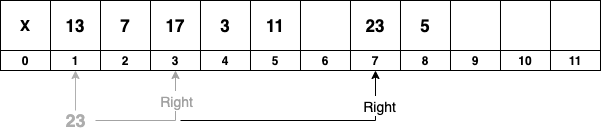
\includegraphics[scale=.4]{images/binary_tree_array_07.png} & 
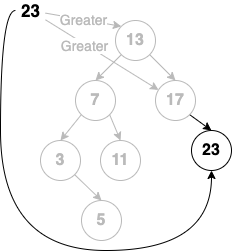
\includegraphics[scale=.4]{images/binary_tree_example_07.png}\\
& \footnotesize{23 is greater than 13, go right. 23 is greater than 17, go right. Its empty, store it there.} &   \\
\hline
\end{tabular}
\end{center}
\begin{center}
\begin{tabular}{|M{0.10\textwidth}|M{0.50\textwidth} M{0.35\textwidth}|}
\hline
Done &
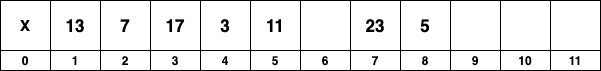
\includegraphics[scale=.4]{images/binary_tree_array_08.png} & 
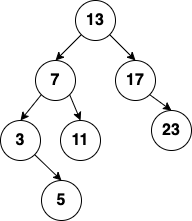
\includegraphics[scale=.4]{images/binary_tree_example_08.png}\\
\hline
\end{tabular}
\end{center}

You can see the resulting array and tree above. Notice the empty slot at index 6. This is the type of thing you want to avoid with array based structures. One empty slot is not a big deal you say? Probably not. However, this is a small forced example. Why don't you continue this example on paper and insert the values 2 then 1. How big did you need to resize your array?\\
